\documentclass[20pt, a0paper, portrait]{tikzposter}

\usepackage[utf8]{inputenc}
\usepackage[T1]{fontenc}
\usepackage{textcomp}
\usepackage{arev}
\usepackage{arevmath}
\usepackage{arevtext}
\usepackage{graphicx}
\usepackage{wrapfig}
\usepackage{microtype}

% Bibliography
\usepackage[backend=biber,
bibencoding=utf8,
bibstyle=numeric-comp,
%style=verbose, %verbose-ibid,
url=true, % include url in reference
doi=true, % include doi in reference
sorting=none, % sorting of citations
%autocite=superscript, % autocite becomes superscript
maxcitenames=1, % Max names displayed when citing in text
maxbibnames=10, % Max number of names displayed in the bibliography
giveninits=true % Use initials
]{biblatex}
\addbibresource{citations.bib}
\renewcommand*{\bibfont}{\footnotesize}

\renewcommand*\familydefault{\sfdefault}

\title{2nd Year Mechanism Design}
\author{Engineering Design \& Manufacture Group}
\date{\today}
\institute{University of Bath, UK}

\usetheme{Default}
\usecolorstyle[colorPalette=GreenGrayViolet]{Default}
\useblockstyle{Default}
\usetitlestyle{Filled}
  
\begin{document}

\maketitle

\block[]{Design Brief}{
  \begin{wrapfigure}{r}{0.65\textwidth}
    \begin{tabular}{c c}
      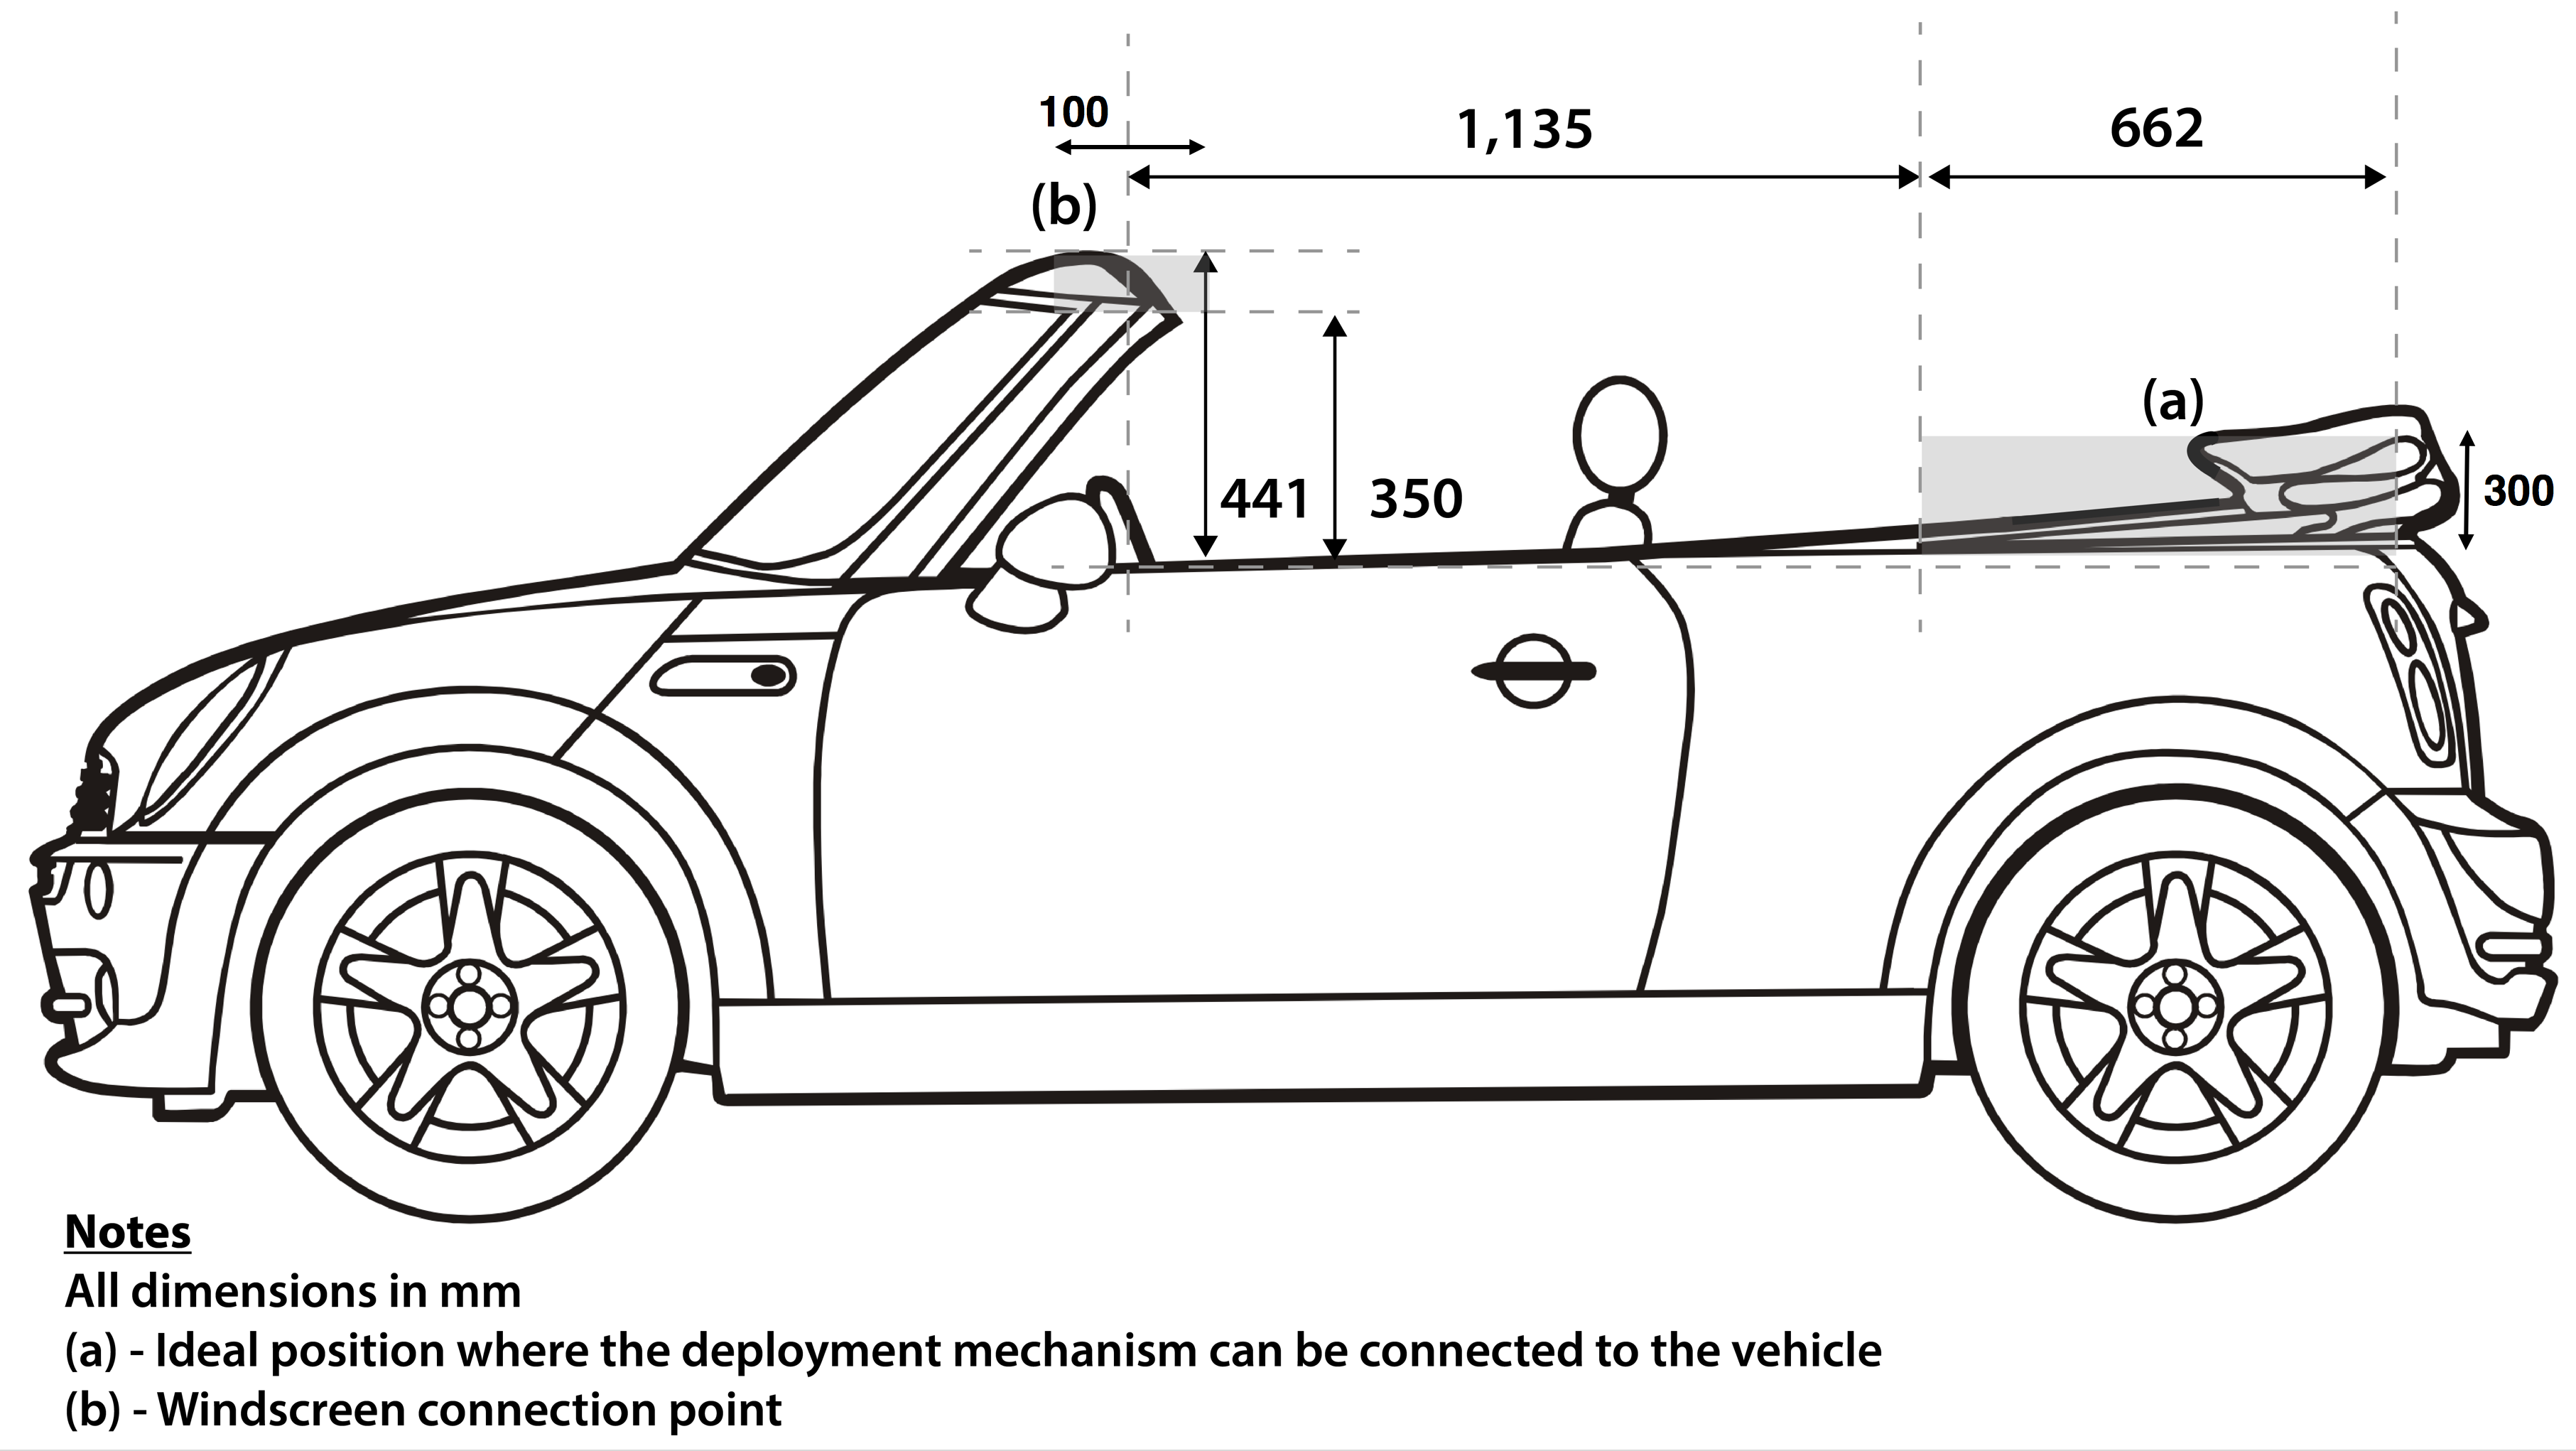
\includegraphics[width=0.3\textwidth]{figures/MiniDimensions.png} &
      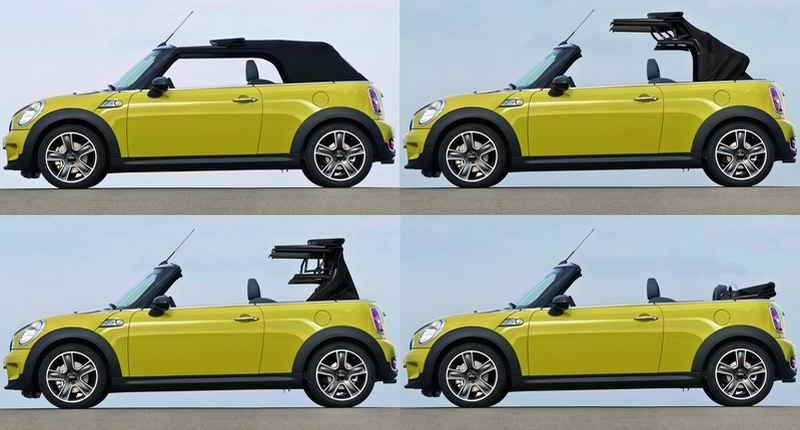
\includegraphics[width=0.3\textwidth]{figures/roof.jpg}
      \\
    \end{tabular}
    \label{fig-roof}
    %\caption{Convertible Roof Design Problem}
  \end{wrapfigure}
  ~\\
  You will be working in groups of \textbf{two} to design a mechanism that will open and close a roof for the convertible car shown in Figure~\ref{fig-roof}. This is an open-ended feasibility exercise with a high level of uncertainty. There are many ways that one could solve the problem. Your report should detail the:

  \vspace{1em}

  \begin{itemize}
    \item design process you have gone through;
    \item assumptions made and their implications; and,
    \item justification for your design decisions.
  \end{itemize}

  \vspace{5cm}
}

\block[]{Requirements Capture, Concept Generation \& Initial Calculations}{
  Students work in groups to research engineering resources (such as, anthropological data) and perform competitor analysis to build a set of requirements that their design must meet. They then continue into the development of some concepts using a number of digital and physical tools. This is followed by a quantitative and qualitative assessment of their concepts against their requirements.
  \begin{tikzfigure}
    \centering
    \begin{tabular}{c c c}
      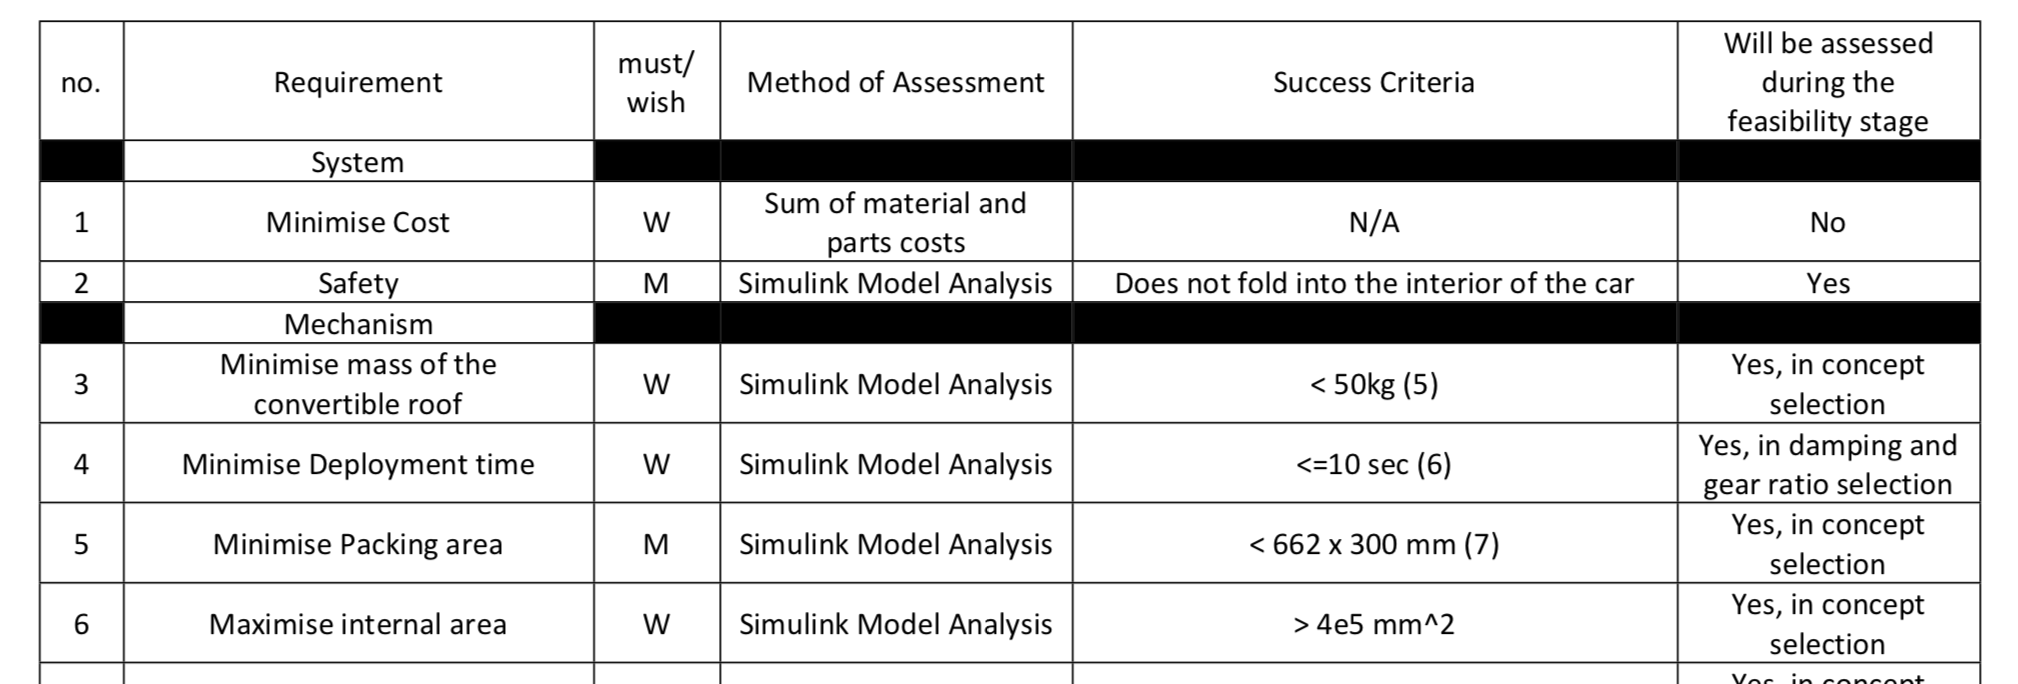
\includegraphics[width=0.4\textwidth]{figures/pds.png} &
      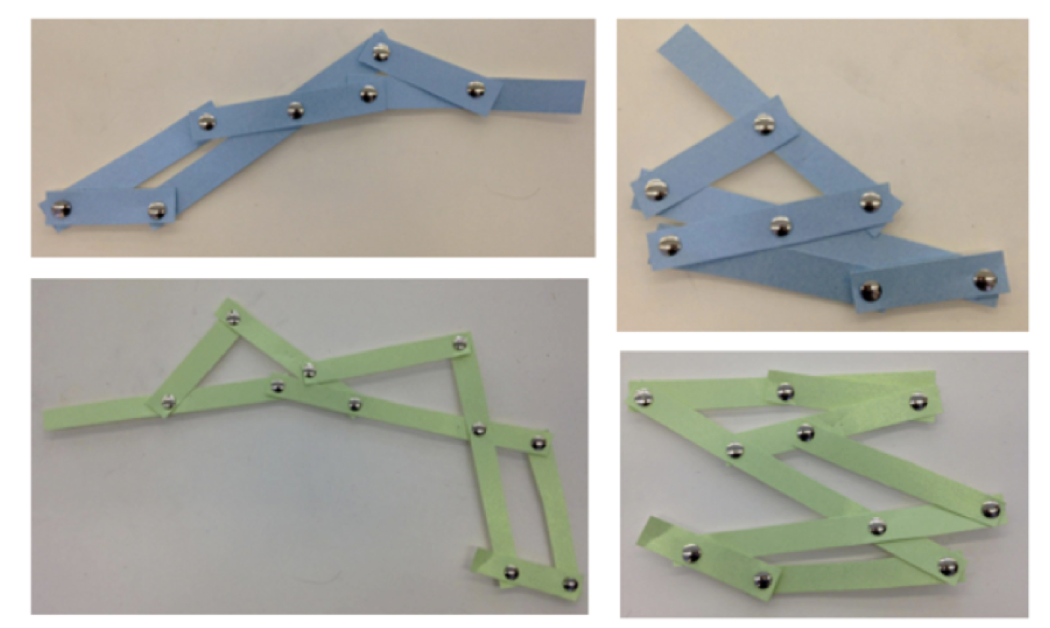
\includegraphics[width=0.25\textwidth]{figures/concepts.png} & 
      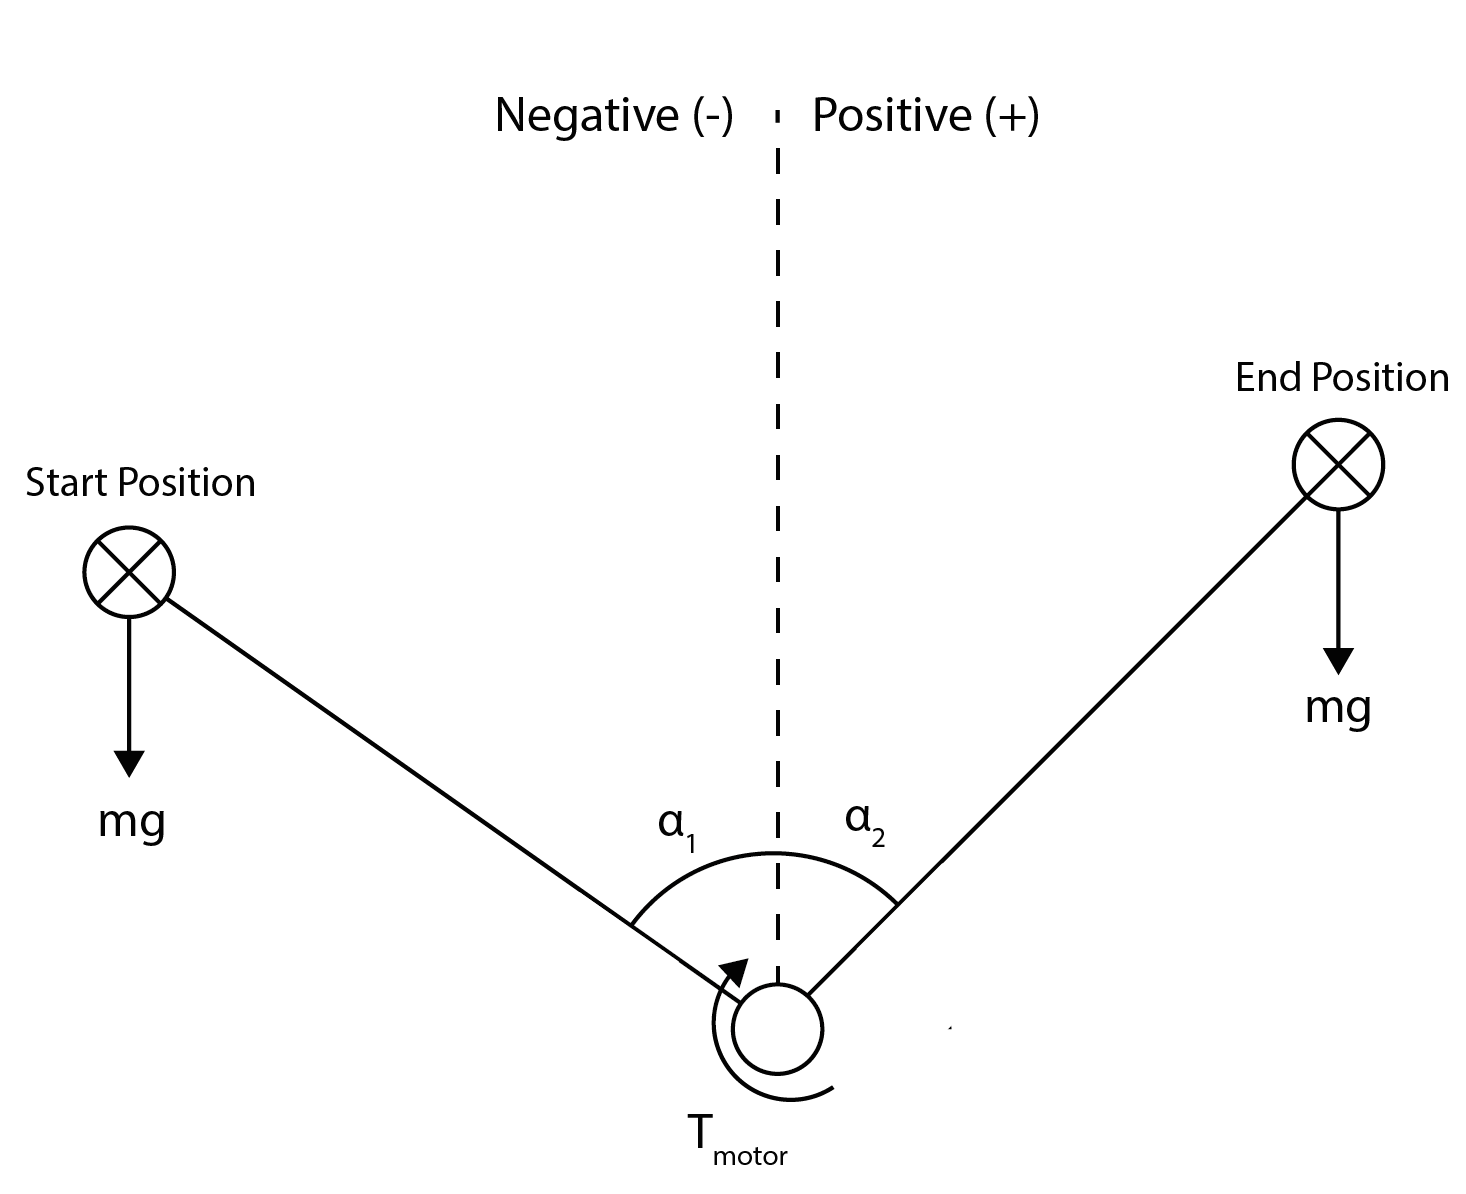
\includegraphics[width=0.2\textwidth]{figures/pendulum.png} \\
      &
      &
      $T_mG > Mgr\sin\theta$$ \\
    \end{tabular}
    %\label{fig-roof}
    %\caption{Convertible Roof Design Problem}
  \end{tikzfigure}
}


\begin{columns}
  \column{0.7}
  \block[]{Full Deployment Simulation}{
    The students then continue to build a full parametric systems model of the mechanism along with the gearbox and motor that will power it. The exercise develop both their analytical and numerical reasoning skills in a practical design exercise.
    \begin{tikzfigure}[]
      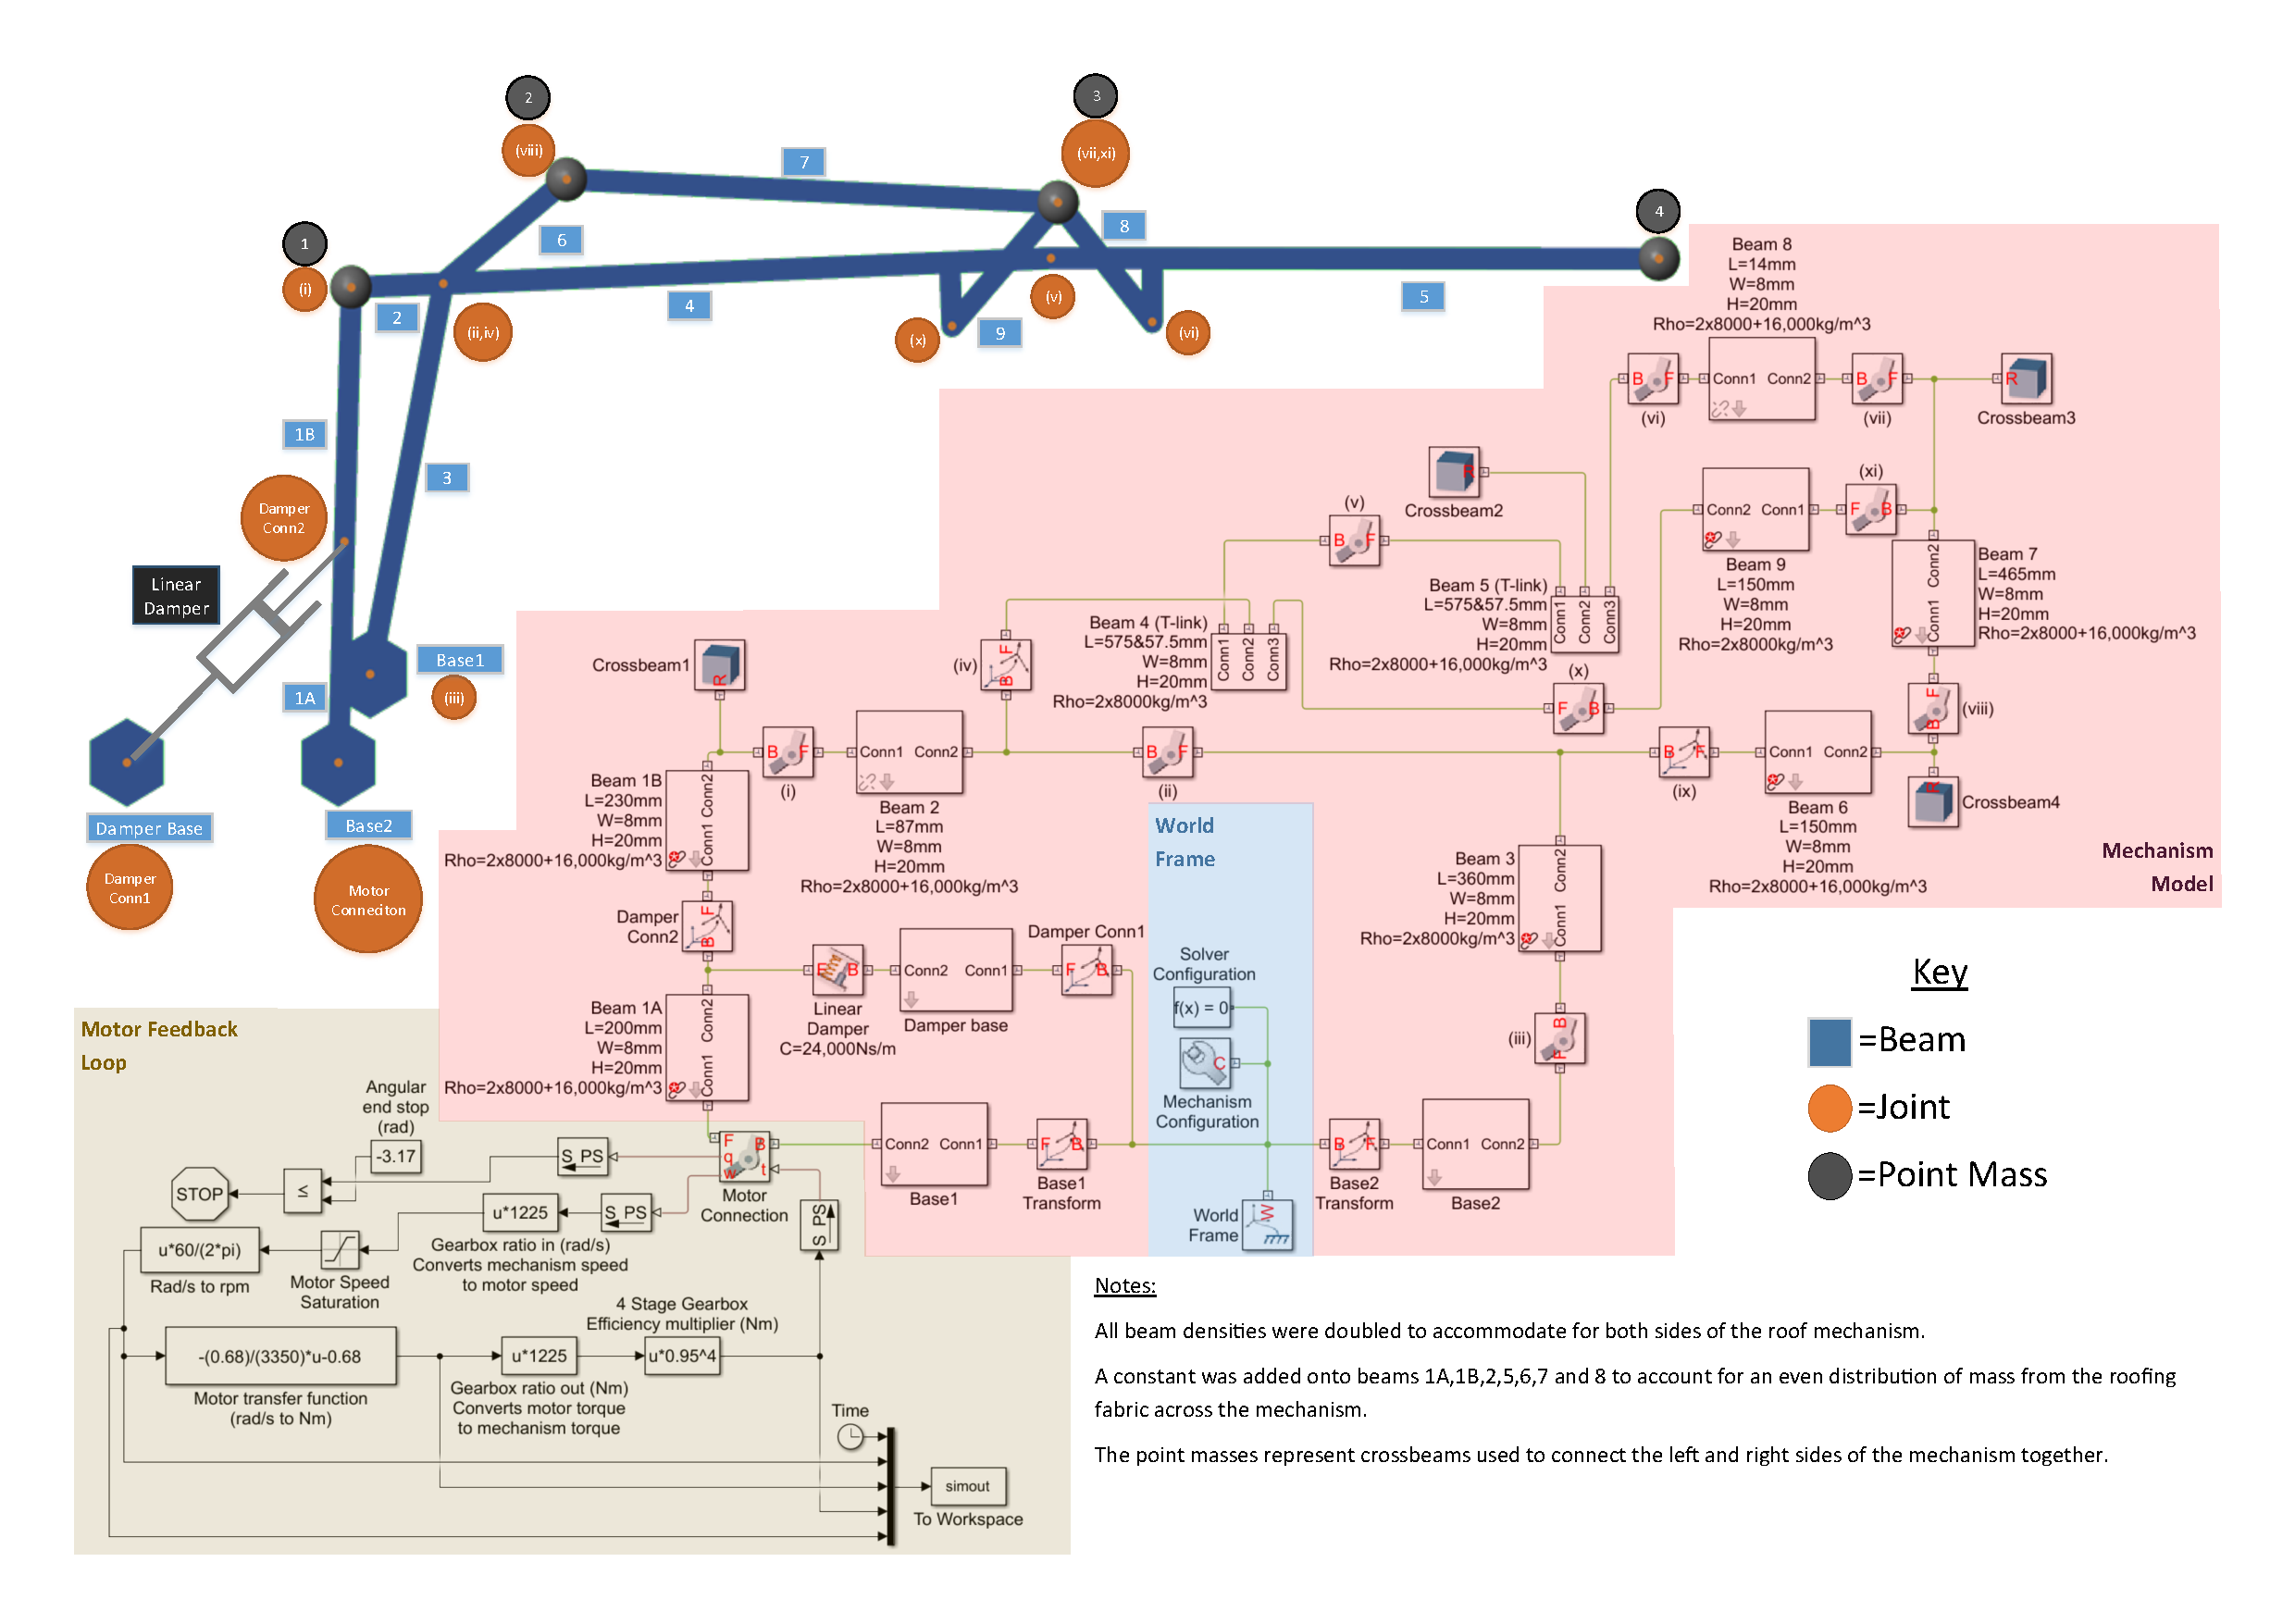
\includegraphics[width=0.65\textwidth]{figures/simulation.pdf}
    \end{tikzfigure}
  }

  \column{0.3}
  \block[]{Results}{
    Using this model, the students evaluate how changing bar positions, motor, gear ratios and damping effect the performance of their convertible roof concept.
    \begin{tikzfigure}[]
      \begin{tabular}{c}
        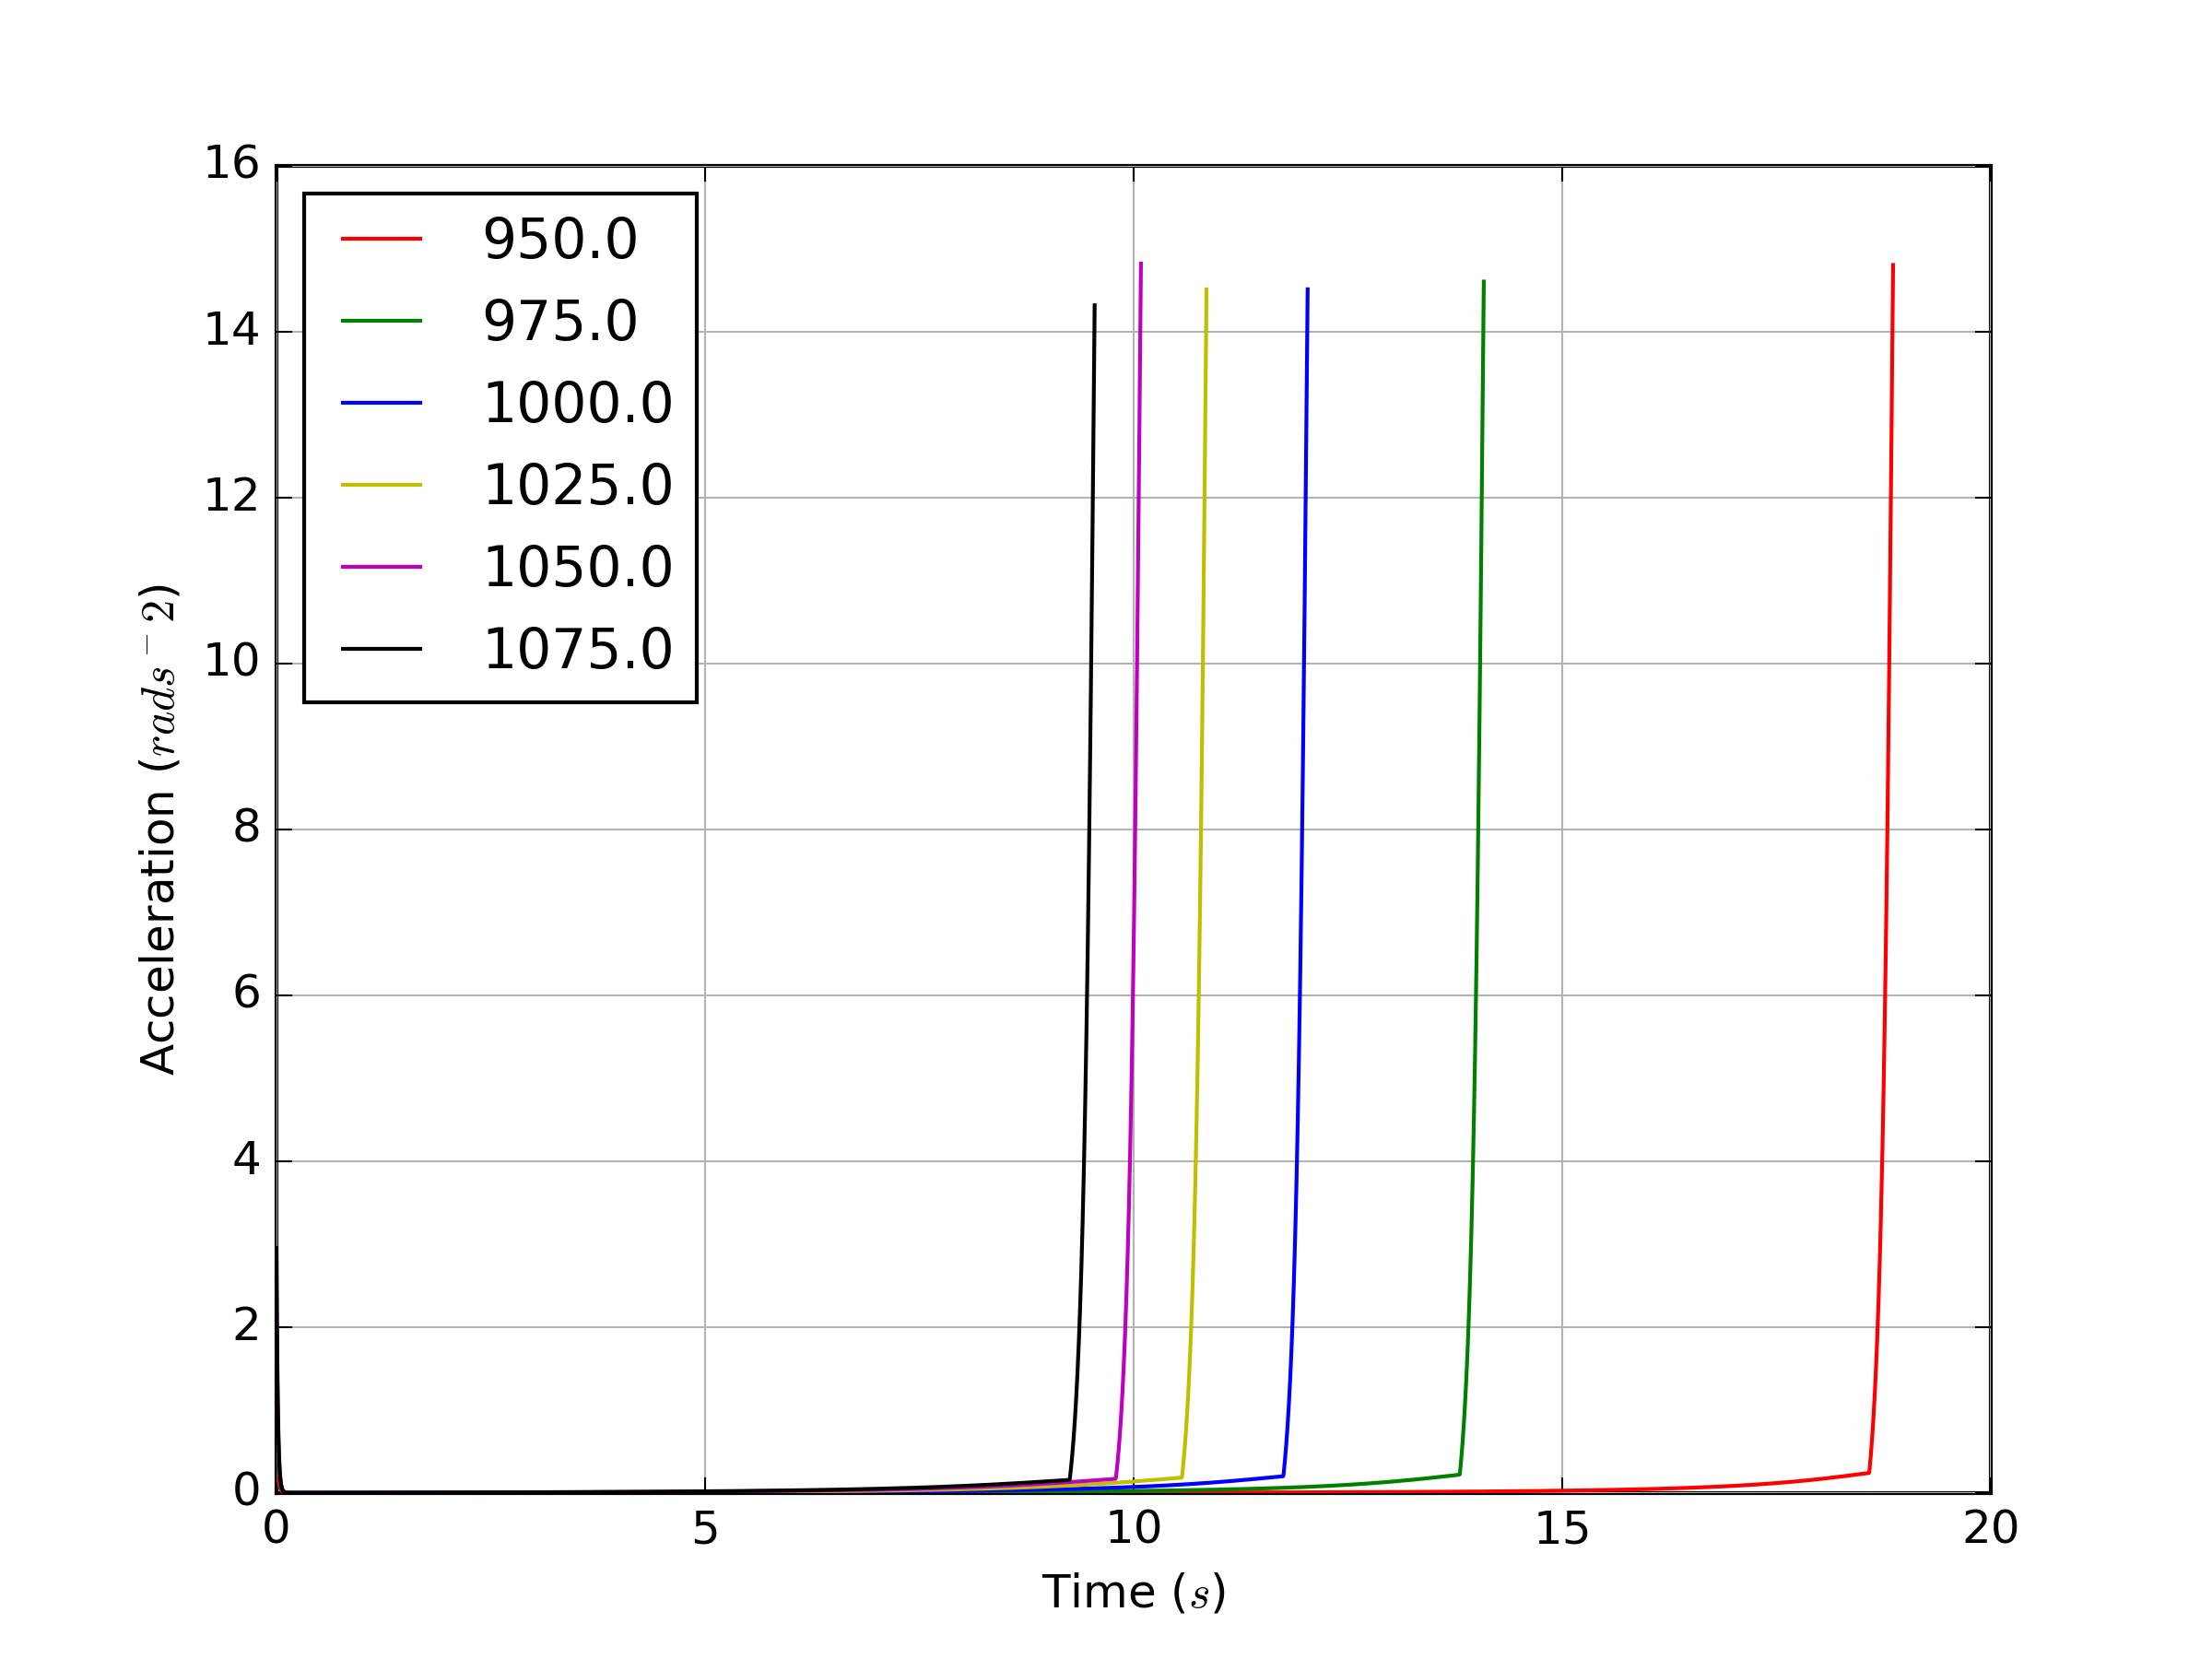
\includegraphics[width=0.2\textwidth]{figures/mechanism_acceleration.png} \\
        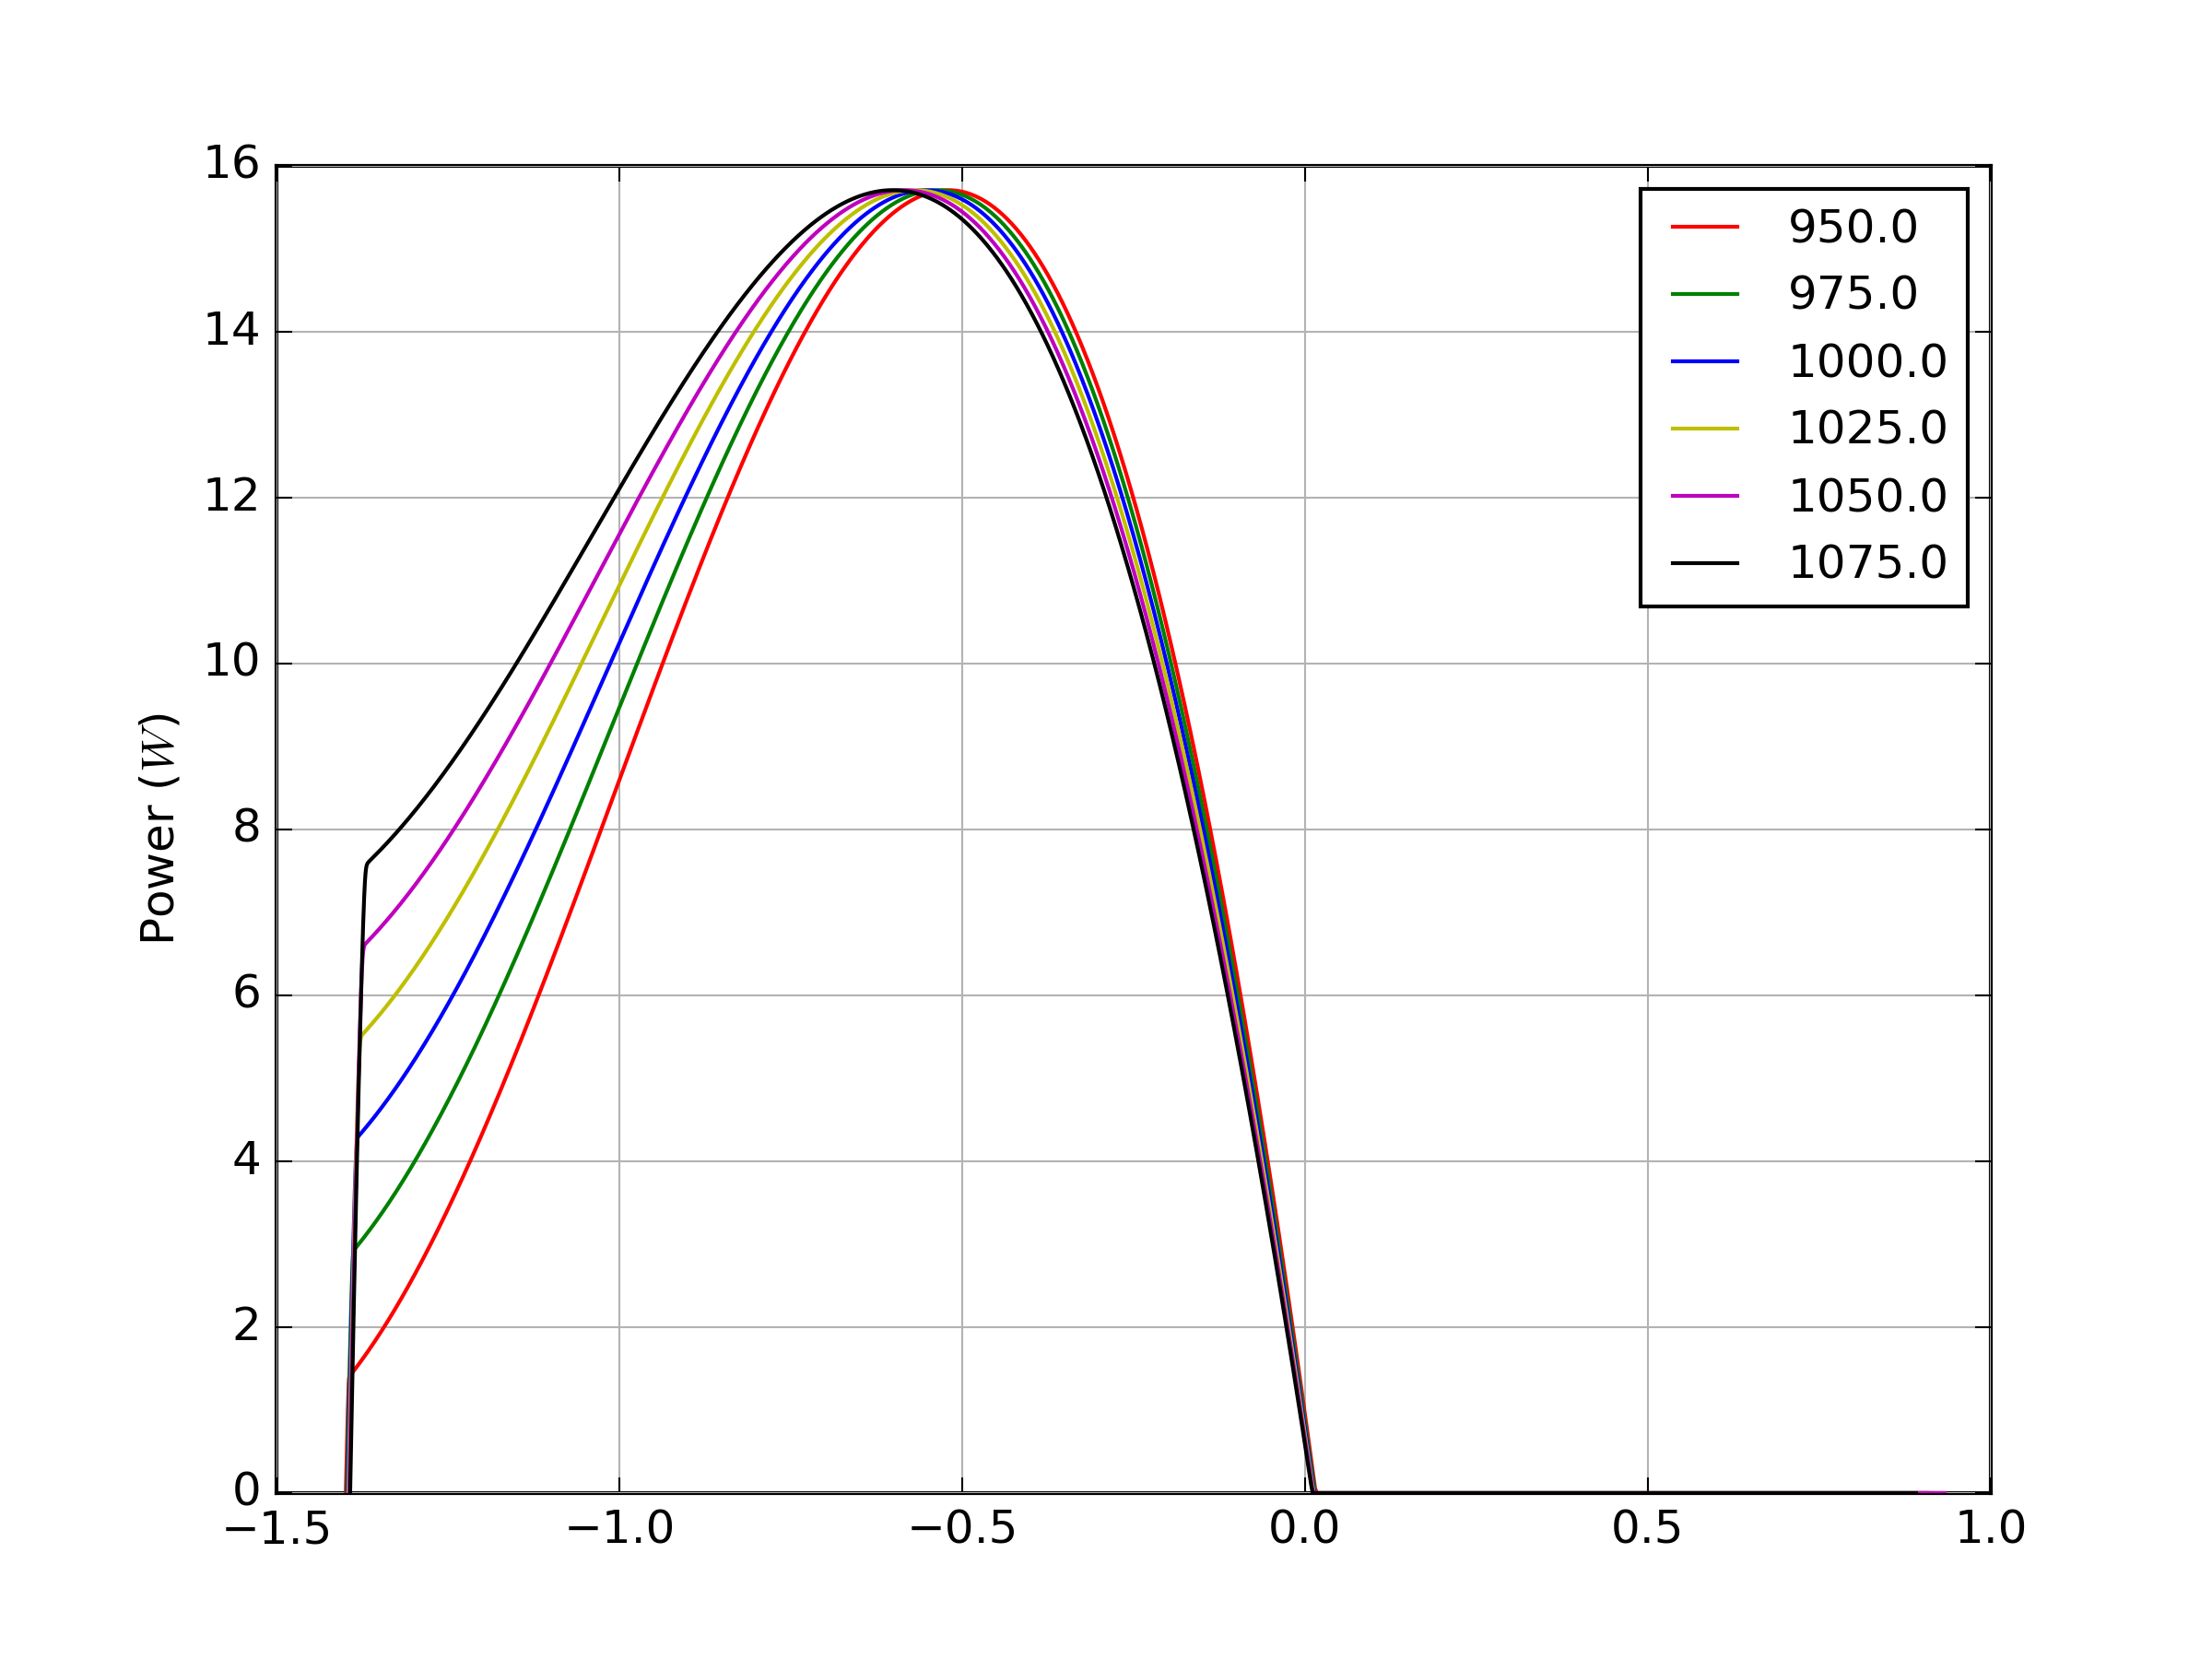
\includegraphics[width=0.2\textwidth]{figures/mechanism_power_angle.png} \\ 
        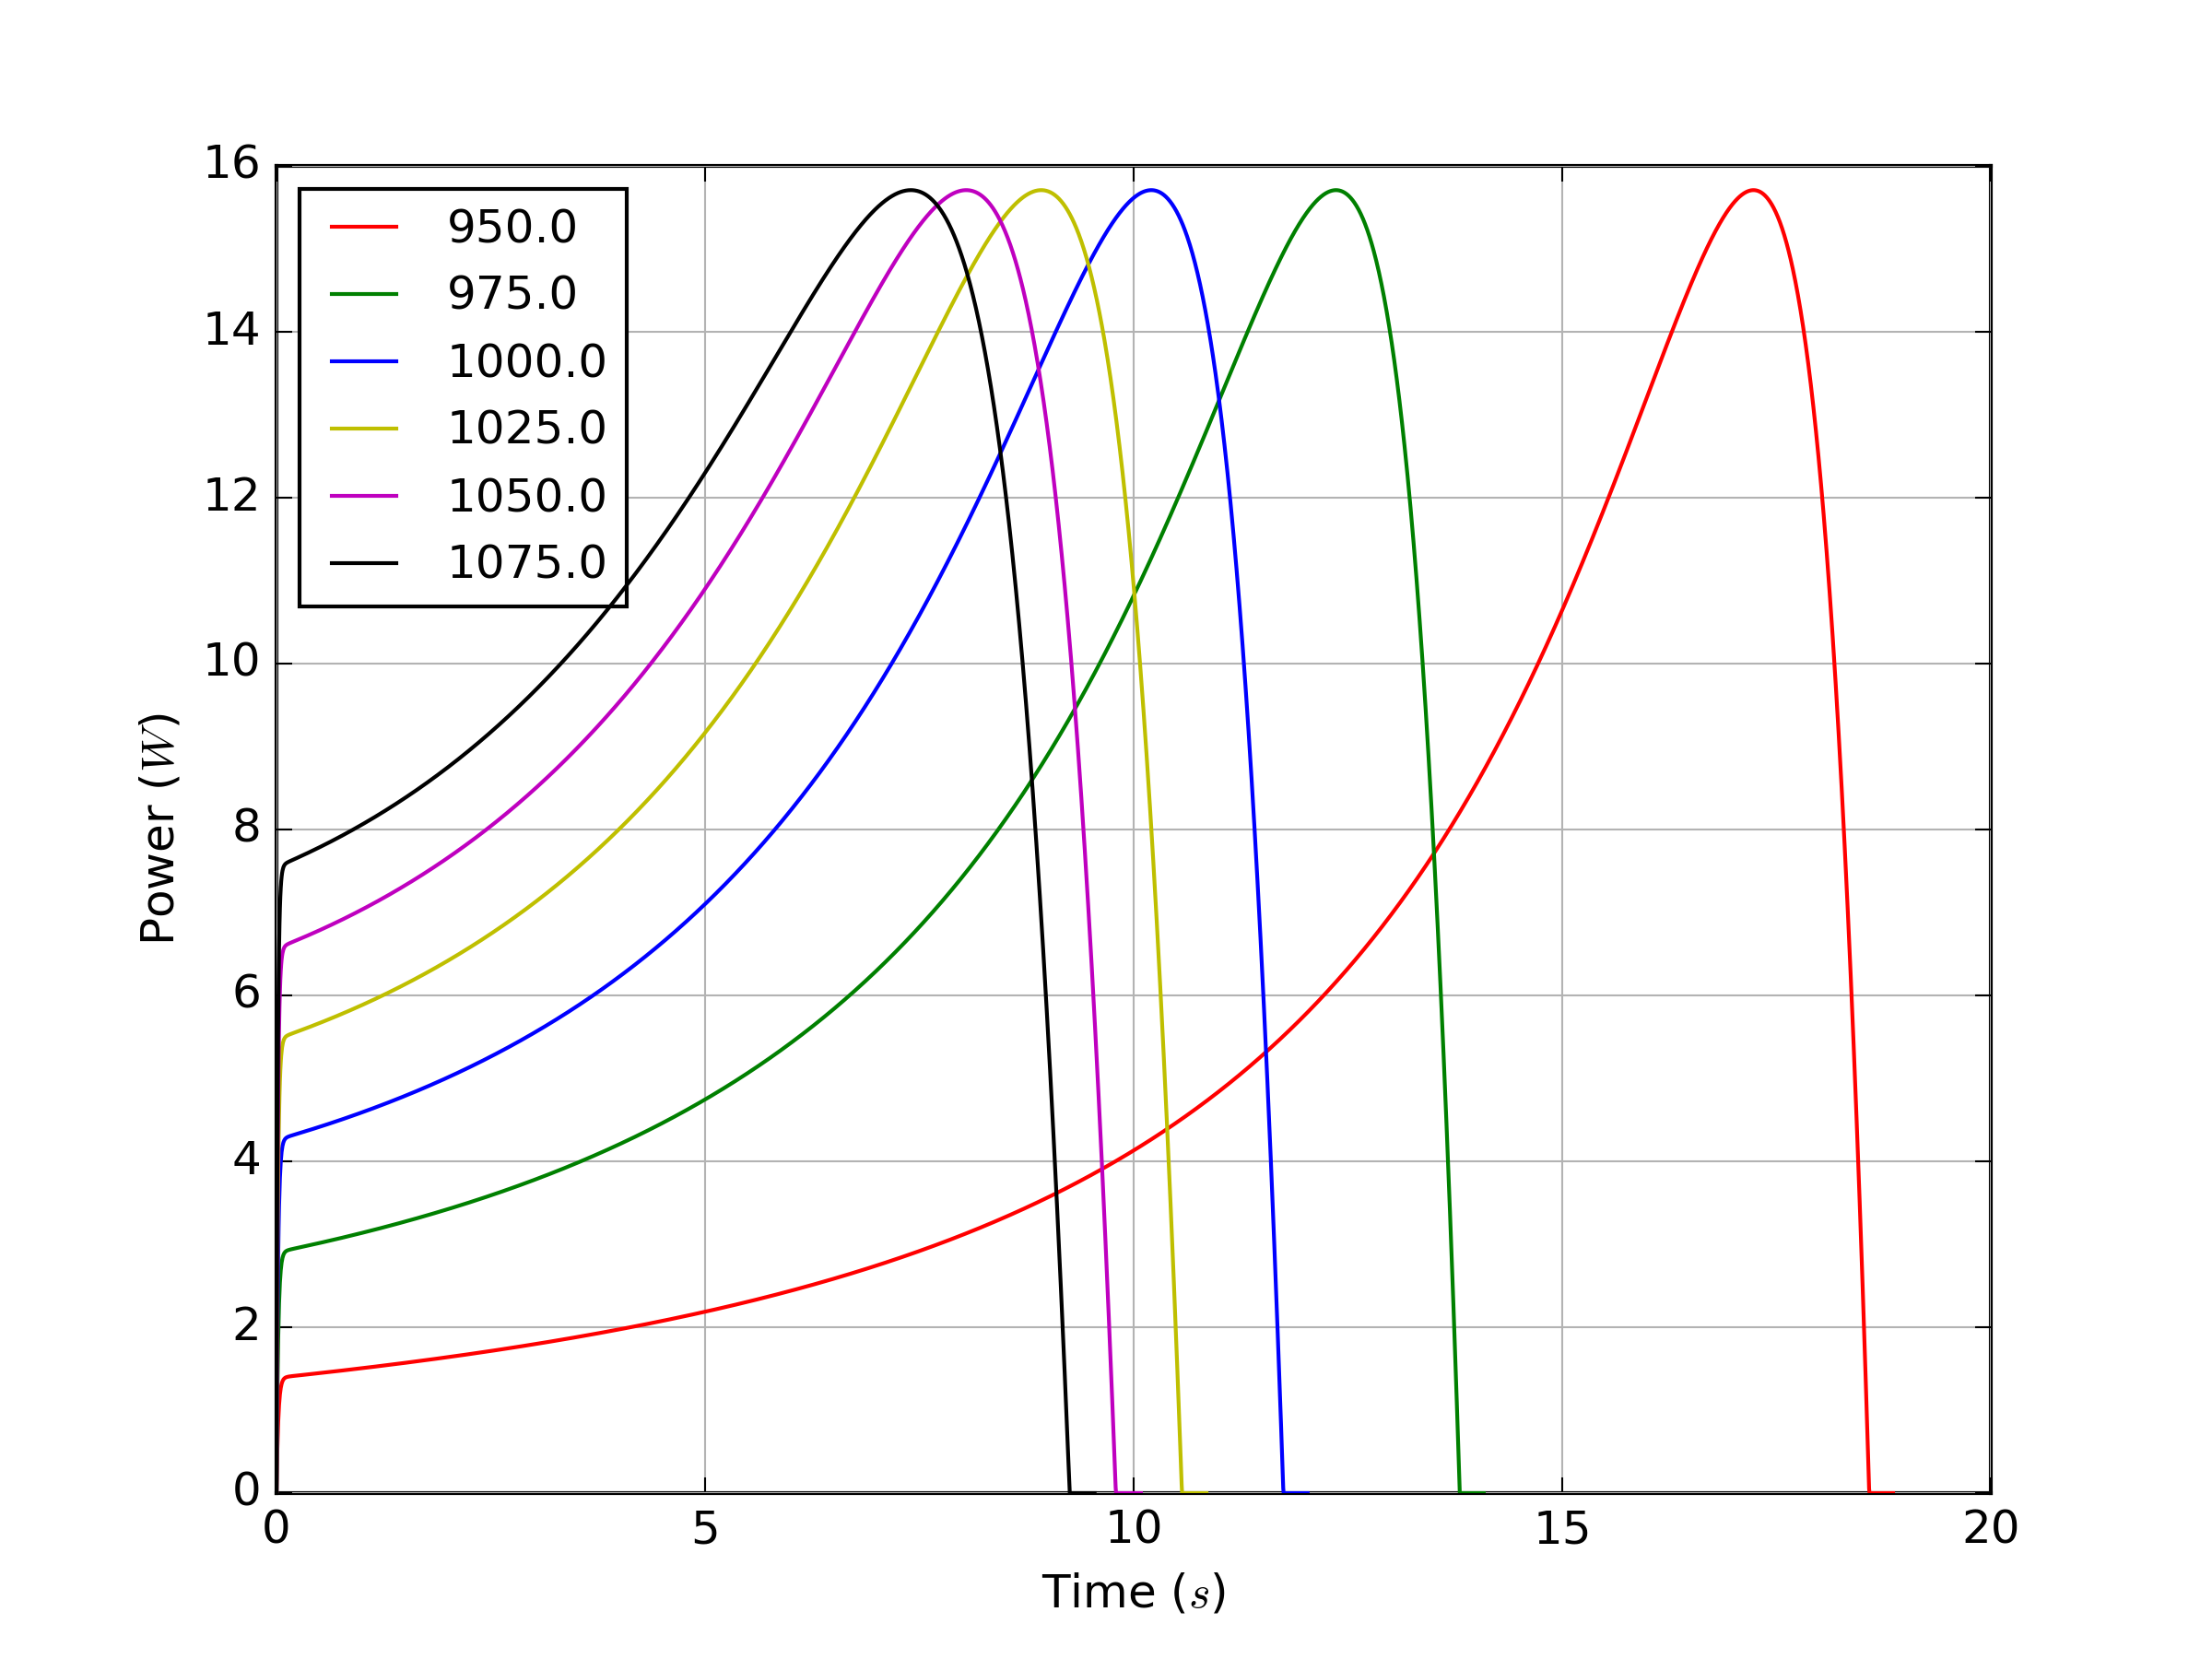
\includegraphics[width=0.2\textwidth]{figures/mechanism_power.png} \\
      \end{tabular}
    \end{tikzfigure}
  }
\end{columns}

\end{document}